\documentclass[preprint,12pt]{elsarticle}

\usepackage[T1]{fontenc}
\usepackage[utf8]{inputenc}
\usepackage[english]{babel}
\usepackage{amsmath,amssymb}
\usepackage{graphicx}
\usepackage{booktabs}
\usepackage{array}
\usepackage{multirow}
\usepackage{xcolor}
\usepackage{hyperref}

\journal{Computerized Medical Imaging and Graphics}

\begin{document}
\begin{frontmatter}

\title{Detection-Guided Adaptive 2D Synthesis for Patient-Level Lung Malignancy Assessment from CT Volumes}

\author[1]{Domenico Paolo\corref{cor1}}
\author[1]{Marco Cantone}
\author[1]{Ciro Russo}
\author[1]{Claudio Marrocco}
\author[1]{Alessandro Bria}

\affiliation[1]{
    organization={Department of Electrical and Information Engineering, University of Cassino and Southern Latium},
    country={Italy}
}

\cortext[cor1]{Corresponding author}

\begin{abstract}
Patient-level malignancy assessment from lung CT constitutes a sparse-evidence aggregation problem, in which discriminative abnormalities occupy only a small fraction of the volumetric input while the supervision and prediction target are defined at the examination level. Integrating such sparse evidence from pulmonary nodules distributed across a three-dimensional examination is therefore challenging~\cite{carbonneau2018multiple}. Full-volume 3D neural networks preserve volumetric context, but their computational and memory requirements constrain resolution, batch size, and practical deployment. Conversely, fixed 2D projections and slice-selection strategies are efficient but may miss or dilute the sparse lesion-level evidence required for a reliable patient-level decision. Thus, an effective representation should retain the efficiency of 2D processing while explicitly preserving and aggregating the spatially distributed abnormalities that determine the examination-level label.

We propose a detection-guided adaptive synthesis framework specifically designed to address this problem by converting a CT volume into a compact patient-specific 2D representation that concentrates sparse lesion evidence. A 3D nodule detector first localizes candidate nodules, identifying the regions most likely to carry discriminative information. The highest-confidence detections are then used as semantic control points for a radial basis function (RBF) surface, which adaptively traverses the volume according to the spatial distribution of the detected lesions. Sampling the preprocessed CT volume along this smooth surface brings otherwise distant nodular abnormalities into a single synthetic 2D image, enabling their joint consideration by standard 2D classifiers while avoiding exhaustive full-volume processing. In this way, the proposed representation directly bridges local lesion localization and global patient-level classification.

On LUNA16, using CPMNetv2 detections with threshold $0.50$ and top-$4$ candidates, the proposed Adaptive RBF representation with EfficientNetV2-S achieved a pooled AUC of $0.8149$ over 796 labeled scans in 10-fold cross-validation. It significantly outperformed MIP axial projection (AUC $0.6075$), MIP tri-view (AUC $0.6175$), central axial slice selection (AUC $0.6153$), detector-crop MIL attention (AUC $0.5410$), fixed/random control-point ablations, and a full-volume 3D ResNet18 baseline (AUC $0.5659$). Paired DeLong tests confirmed significant AUC improvements over all planned comparators after FDR correction. These results indicate that the proposed framework effectively addresses the sparse-evidence aggregation problem by selectively concentrating spatially distributed lesion information into a compact representation suitable for global patient-level classification, rather than benefiting merely from dimensionality reduction.
\end{abstract}

\begin{keyword}
Lung CT \sep Patient-level malignancy \sep Detection-guided synthesis \sep Adaptive projection \sep Radial basis functions
\end{keyword}

\end{frontmatter}

\section{Introduction}

Low-dose computed tomography (CT) plays a central role in lung cancer screening, with randomized trials demonstrating a reduction in lung-cancer mortality compared with radiography or no screening~\cite{nlst2011,nelson2020}. From a computational perspective, however, CT presents a difficult imbalance between the size of the input and the amount of clinically relevant information it contains. A screening examination may span hundreds of slices, whereas only a limited number of small pulmonary nodules may contribute meaningfully to the final assessment~\cite{armato2011lidc,setio2017luna16}. The relevant findings may also appear at distant spatial locations within the same scan. Consequently, a patient-level model must identify a small set of informative regions and combine them into a single decision while remaining robust to the much larger amount of non-informative anatomy.

Existing deep learning strategies approach this challenge in different ways. Volumetric architectures retain three-dimensional anatomical context and have been successfully explored for pulmonary nodule characterization and lung cancer risk prediction~\cite{zhu2018deeplung,ardila2019endtoend,mikhael2023sybil}, but dense 3D processing is computationally and memory intensive. Conversely, fixed projections, selected slices, and multi-view representations reduce computational cost and allow the use of efficient 2D backbones~\cite{setio2016multiview,zheng2020mip,jang2022m3t}. Their sampling geometry, however, does not adapt to the lesion configuration of each patient, so small or spatially separated nodules may be missed or diluted. Local crop-based approaches preserve candidate lesions more explicitly, but require a separate aggregation mechanism to obtain a patient-level prediction, as in multiple-instance learning~\cite{ilse2018attention}.

We therefore investigate whether lesion localization can guide the construction of a compact representation tailored to each examination. A 3D nodule detector from the center-points matching family~\cite{song2020cpm,luo2022scpmnet} first identifies candidate abnormalities. High-confidence detections are then used as control points for a smooth radial basis function (RBF) surface~\cite{powell1987rbf}, whose geometry adapts to the spatial distribution of the detected nodules. Sampling the CT volume along this surface produces a single synthetic 2D image that brings spatially separated abnormalities into a common representation while retaining surrounding anatomical context.

This formulation separates lesion localization from final classification while preserving a direct connection between the two. The detector determines where relevant evidence is likely to be located, the adaptive surface determines how this evidence is represented, and a standard 2D backbone performs the examination-level prediction. Importantly, the intermediate representation is explicit rather than latent: the synthesized image can be directly inspected together with the detected candidates and control points, enabling qualitative assessment of which portions of the original volume are retained before classification.

The main contributions of this work are:
\begin{itemize}
\item We introduce a detection-guided adaptive 3D-to-2D representation for patient-level lung malignancy assessment, designed to gather spatially separated lesion evidence into a single image.

\item We use detector-derived control points to construct a patient-specific RBF sampling surface, allowing the sampling geometry to adapt to the lesion configuration of each CT examination.

\item We provide the synthesized 2D image as an explicit and directly inspectable intermediate output between lesion localization and patient-level classification.

\item We compare the proposed strategy with fixed 2D projections and slice-selection baselines, detector-crop multiple-instance learning, fixed and random control-point variants, Shepard interpolation, and a full-volume 3D ResNet18 model.

\item We complement predictive evaluation with paired statistical testing and computational analysis, distinguishing downstream classification cost from detector-inclusive processing.

\end{itemize}


\section{Related Work}

\subsection{Volumetric lung CT analysis}

Deep learning methods for lung CT have increasingly exploited volumetric representations to preserve the three-dimensional structure of pulmonary findings. DeepLung combined 3D nodule detection with volumetric feature extraction for nodule diagnosis~\cite{zhu2018deeplung}. Subsequent end-to-end systems showed that whole CT examinations can support patient-level lung cancer risk prediction from current and prior scans~\cite{ardila2019endtoend}, while Sybil demonstrated multi-year risk estimation from a single low-dose CT~\cite{mikhael2023sybil}. These approaches highlight the value of volumetric context, but they also require processing large amounts of anatomy that may not directly contribute to the prediction. This is particularly relevant in lung CT, where discriminative abnormalities can be sparse relative to the overall examination. Dense 3D processing therefore remains computationally and memory intensive, especially when high-resolution inputs are required.

\subsection{2D projections and multi-view representations}

Reduced-dimensional representations provide a more computationally efficient alternative to full-volume processing. Multi-view CNNs have been used for pulmonary nodule false-positive reduction~\cite{setio2016multiview}, while hybrid 2D/3D architectures aggregate information across multiple planes or slices~\cite{jang2022m3t}. Maximum intensity projections (MIPs) are also relevant in lung imaging because high-attenuation nodules can be emphasized relative to surrounding lung parenchyma~\cite{zheng2020mip}.

These approaches reduce the dimensionality of the input before classification, but their sampling geometry is generally fixed across patients. Consequently, the representation is not explicitly conditioned on the location of the abnormalities that may determine the examination-level label. Small nodules can be attenuated or omitted, while spatially separated findings may be represented inefficiently within the same projection. Our approach retains the computational advantages of 2D classification but makes the volumetric sampling strategy dependent on the detected lesion configuration of each examination.

\subsection{Detection-guided patient-level reasoning}

Lesion detection provides a natural way to focus computation on the small subset of regions that are more likely to contain discriminative information. SCPM-Net models pulmonary nodules through center-point matching and represents detected lesions as bounding spheres~\cite{luo2022scpmnet}. CPMNetv2 extends this detector family with further training and inference refinements.

Once candidate nodules have been identified, a common strategy for patient-level reasoning is to process them individually and aggregate their representations through mean, max, or attention-based pooling, as in multiple-instance learning~\cite{ilse2018attention}. Such methods perform aggregation primarily in feature or decision space. In contrast, our method uses the detected candidates to guide the construction of a shared image representation before classification. Spatially separated lesions are therefore presented jointly to the downstream model, together with portions of their surrounding anatomical context.

This distinction is also relevant from an interpretability perspective. Candidate-based MIL approaches typically aggregate latent representations, whereas our pipeline produces an explicit intermediate image that can be visually inspected before the final classifier is applied. The synthesized representation therefore provides a direct connection between lesion localization, adaptive sampling, and examination-level prediction.

\subsection{Adaptive geometric synthesis}

Radial basis functions provide a classical framework for interpolating smooth functions from scattered observations. Thin-plate spline formulations, in particular, have been widely used to model smooth non-rigid transformations in image analysis and computer vision~\cite{bookstein1989principal,cantone2025deep}. Given sparse control points and associated target coordinates, they define a continuous surface whose shape depends globally on the spatial configuration of those points.

In our setting, detector-selected nodules provide semantically meaningful control points rather than generic geometric landmarks. The resulting surface is used to determine which axial locations should be sampled across the CT volume, thereby converting a sparse set of three-dimensional lesion locations into a dense two-dimensional representation.

We also consider Shepard interpolation~\cite{shepard1968} as an alternative adaptive strategy. Unlike thin-plate RBF interpolation, which derives a globally coupled surface from all control points, Shepard interpolation estimates each location through inverse-distance weighting and therefore emphasizes nearby control points. Using the same detector-selected candidates for both formulations allows us to compare different interpolation mechanisms while keeping lesion guidance unchanged.

\section{Materials and Methods}

\subsection{Dataset, labels, and preprocessing}

Experiments were performed on LUNA16~\cite{setio2017luna16}, a curated subset of LIDC-IDRI~\cite{armato2011lidc}. LUNA16 contains 888 CT scans and 1,186 reference nodules with diameter at least 3 mm accepted by at least three of four radiologists.

Because LUNA16 is primarily a nodule-detection benchmark, patient-level malignancy labels were derived from the corresponding LIDC-IDRI radiologist ratings. For each annotated nodule, the malignancy scores assigned by the radiologists were averaged. The maximum mean malignancy score across all nodules in a scan was then used to define the examination-level label: scans with a score below 3 were labeled benign, those with a score above 3 were labeled malignant, and scans with a score equal to 3 were excluded as indeterminate. This procedure resulted in 796 labeled scans, including 320 malignant and 476 benign cases.

The original LUNA16 \texttt{.mhd/.raw} volumes were converted to NIfTI format and standardized using SimpleITK. Each scan was resampled to isotropic $1.0 \times 1.0 \times 1.0$ mm spacing with linear interpolation. CT intensities were clipped to the lung window $[-1200,600]$ HU and linearly mapped to $[0,255]$. Lung masks were obtained using the \texttt{lungmask} R231 model, dilated by 10 iterations, and used to suppress non-lung regions. A three-dimensional bounding box around the lung mask was expanded by 10 voxels in each direction and used to crop the CT volume. When lung segmentation failed, the full resampled volume was retained.

Official LUNA16 annotations were read from \texttt{annotations.csv}. Nodule centers were transformed from world coordinates to the voxel space of the processed CT volume while preserving image origin, spacing, and direction. Annotation diameters were used to generate spherical binary nodule masks. For each scan, the preprocessing pipeline stored the processed CT volume, lung mask, nodule mask, and associated metadata, together with a global CSV file containing nodule coordinates and sizes in the processed image space.

Figure~\ref{fig:dataset_overview} shows representative benign and malignant examinations and illustrates the volumetric structure of the data, the distribution of nodules across axial slices, and representative lesion appearances.

\begin{figure*}[t]
\centering
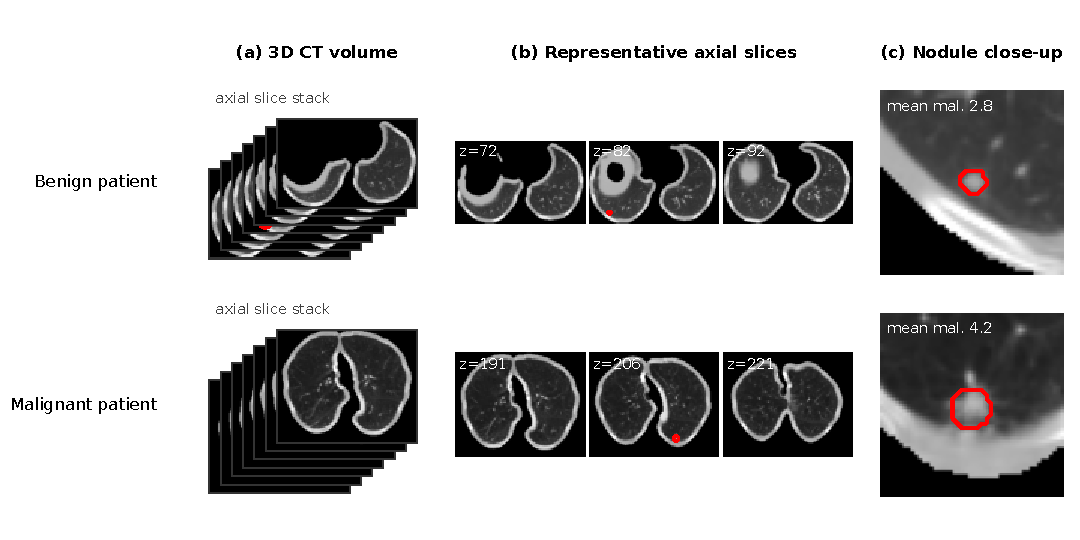
\includegraphics[width=\textwidth]{figures/dataset_overview_representative_cases.pdf}
\caption{
Representative benign and malignant cases from the LUNA16/LIDC-IDRI dataset.
For each examination, the figure shows the CT volume as an axial slice stack,
representative axial slices around an annotated pulmonary nodule, and a close-up
of the corresponding lesion with the ground-truth annotation.
The reported malignancy score corresponds to the mean LIDC-IDRI malignancy rating
associated with the selected nodule.
}
\label{fig:dataset_overview}
\end{figure*}

\subsection{Detector and working point}

We used CPMNetv2 as the nodule detector and evaluated it with 10-fold cross-validation on LUNA16. In each fold, the detector was trained on the corresponding training subsets and evaluated on the held-out test subset, so each scan contributed once to the final test evaluation. The detector outputs candidate centers, radii, and probabilities in the preprocessed voxel space. For the pooled FROC analysis, predictions and reference nodules from the 10 held-out test subsets were concatenated, yielding a dataset-level evaluation over the full LUNA16 cohort. Table~\ref{tab:detector_froc} reports sensitivity at the seven standard LUNA16 false-positive rates: $0.125$, $0.25$, $0.5$, $1$, $2$, $4$, and $8$ FP/scan. The pooled mean FROC, computed as the average sensitivity over these seven operating points, was $0.8017$.

\begin{table}[t]
\centering
\caption{Pooled CPMNetv2 FROC on LUNA16 over the 10 held-out test folds. Mean FROC is the average sensitivity over the seven listed FP/scan operating points.}
\label{tab:detector_froc}
\begin{tabular}{lrrrrrrr}
\toprule
FP/scan & 0.125 & 0.25 & 0.5 & 1 & 2 & 4 & 8 \\
\midrule
Sensitivity & 0.499 & 0.644 & 0.765 & 0.852 & 0.921 & 0.954 & 0.977 \\
\bottomrule
\end{tabular}
\end{table}

For the subsequent synthesis stage, the detector operating point was selected according to a representation-budget criterion derived from the nodule burden observed in the dataset, rather than by maximizing detection sensitivity alone. This distinction is important because each retained detection defines a geometric control region for the adaptive sampling surface. Consequently, false-positive detections are not merely additional candidates: they may redirect the surface toward non-informative anatomical regions and dilute the lesion-related evidence encoded in the final 2D representation.

To define the maximum number of detector candidates retained per scan, we used the empirical distribution of annotated nodules in LUNA16. The dataset contains on average $1.336$ nodules per scan, with a standard deviation of $1.530$. We therefore defined the representation budget from the descriptive upper range $\mu + 2\sigma$, yielding

\begin{equation}
k_{\mathrm{budget}} = \mu_N + 2\sigma_N
= 1.336 + 2(1.530)
= 4.396.
\end{equation}

Since the number of retained detections must be integer-valued, this criterion was operationalized as a maximum of four detections per scan ($\mathrm{top}\text{-}k=4$). Importantly, $\mu+2\sigma$ is used here as a descriptive, distribution-based heuristic rather than under an assumption of Gaussian nodule counts. Its purpose is to set a representation capacity that accommodates scans with a nodule burden substantially above the dataset mean while preventing the synthesis procedure from being dominated by the small number of scans with unusually large numbers of nodules. In this way, the candidate budget is determined from the characteristics of the dataset independently of downstream classification performance, reducing the possibility of selecting $k$ through task-specific optimization.

After fixing $\mathrm{top}\text{-}k=4$, we adopted a probability threshold of $0.50$, corresponding to the standard decision threshold for probabilistic binary predictions. This provides a simple and reproducible operating point without introducing an additional threshold-tuning step. At this working point, the detector covers 986 of 1,186 annotated nodules ($83.14\%$) and 586 of 601 positive scans ($97.50\%$), while resulting in $2.05$ FP/scan.

\subsection{Adaptive thin-plate RBF synthesis}

For each scan, the detector candidates surviving the selected working point define the primary control regions. Because the synthesized image is generated from a single-valued surface $z=S(x,y)$, two candidates with the same projected $(x,y)$ location but different axial coordinates cannot both be represented at that pixel. We therefore remove projected duplicates before surface fitting, retaining the highest-priority candidate, based on malignancy score when available and otherwise detector probability.

For the proposed RBF representation, every retained detection contributes five control points: the detected center plus four contour points placed on the predicted-radius circle in the axial plane at angles $0$, $\pi/2$, $\pi$, and $3\pi/2$. These points are fitted with a thin-plate spline RBF using smoothing $0.1$. The contour points constrain the fitted surface around the local spatial extent of the candidate rather than only at its center. All control points are clipped to the preprocessed volume bounds.

Let $\mathbf{p}_i=(x_i,y_i)$ denote the projected location of the $i$-th control point and $z_i$ its corresponding axial coordinate. The sampling surface is modeled as

\begin{equation}
S(x,y) =
\sum_{i=1}^{N} w_i\,
\phi\!\left(\left|(x,y)-\mathbf{p}_i\right|\right),
\qquad
\phi(r)=r^2\log(r),
\end{equation}

with the convention $\phi(0)=0$. The coefficients $w_i$ are obtained from the regularized interpolation system defined by the control-point depths, with smoothing parameter $0.1$. The resulting function $S(x,y)$ assigns an axial coordinate to every location in the output image plane.

For comparison, Shepard interpolation uses the same detector-selected candidates and working point while replacing the global thin-plate interpolation rule with inverse-distance weighting. Each retained candidate is represented as a disk centered at $(x_i,y_i,z_i)$ with the predicted detector radius, and overlapping disks in the $(x,y)$ plane are removed before interpolation to avoid assigning conflicting depths to the same projected region. The Shepard surface is defined as

\begin{equation}
S_{\mathrm{Shepard}}(x,y)=
\frac{
\sum_{i=1}^{N} d_i(x,y)^{-p} z_i
}{
\sum_{i=1}^{N} d_i(x,y)^{-p}
},
\qquad
d_i(x,y)=
\left|(x,y)-\mathbf{p}_i\right|.
\end{equation}

In contrast to the globally coupled thin-plate RBF surface, Shepard interpolation gives greater influence to nearby control points and therefore provides an adaptive comparator in which detector guidance is preserved while only the interpolation mechanism is changed.

For both strategies, the estimated surface provides one depth coordinate for each output pixel. The preprocessed CT volume is sampled at these coordinates to generate a single synthetic 2D image. Unless otherwise stated, synthetic images were resized to $256 \times 384$ and represented as three-channel images for compatibility with ImageNet-pretrained backbones.

Figure~\ref{fig:method} illustrates the proposed pipeline: the preprocessed CT volume is processed by a detector, detections are converted into control points, an adaptive thin-plate RBF surface is fitted, and the final synthetic 2D image is classified at the patient level.

\begin{figure}[t]
\centering

\includegraphics[width=\linewidth]{figures/Method.pdf}
\caption{Overview of the proposed detection-guided adaptive synthesis framework. CPMNetv2 identifies candidate nodules in the preprocessed CT volume. The selected detections define control points for a thin-plate RBF surface, which samples the volume to produce a compact synthetic 2D representation for patient-level malignancy classification.}
\label{fig:method}
\end{figure}

\subsection{Baselines and ablations}

To assess the contribution of the proposed detector-guided geometric representation, we compared it with a set of baseline and ablation models. These experiments were designed to disentangle the effect of adaptive lesion localization, multi-view projection, control-point placement, and the interpolation strategy used to generate the final 2D representation.

\begin{itemize}
    \item \textbf{MIP axial and MIP tri-view:} maximum intensity projection baselines computed directly from the preprocessed CT volume. The axial MIP summarizes the volume along a single anatomical direction, whereas the tri-view MIP combines projections from the axial, coronal, and sagittal planes. These baselines provide fixed, non-adaptive 2D representations that do not use detector outputs or lesion-specific spatial information.

    \item \textbf{Central axial slice:} a single 2D slice extracted from the center of the preprocessed volume along the axial axis. This baseline evaluates the performance of a minimal fixed-slice representation, without volumetric aggregation, adaptive projection, or detector-guided localization.

    \item \textbf{Detector crop-MIL:} a detector-guided multiple-instance learning baseline. For each volume, the top-$4$ detector responses were used to extract 2D crops centered on the predicted lesion locations. Each crop was processed independently by the same 2D encoder used in the proposed model, and the resulting features were aggregated through an attention-based MIL module. This baseline preserves detector-guided localization but represents the volume as a sparse set of local image patches rather than as a continuous projected surface.

    \item \textbf{Fixed-control and random-control RBF:} RBF ablations used to test whether performance depends on detector-guided control-point localization. In both cases, the number of candidate regions was matched to the selected detector working point (top-$4$ detections and threshold = $0.5$), while detector-predicted coordinates were replaced by synthetic locations.
    For fixed control, pseudo-detections were placed at predefined normalized in-plane positions with depth fixed to the central slice. For random control, pseudo-detection centers were sampled using a deterministic patient-specific seed, preferentially within the lung mask when available. Radius values were derived from detector candidates, using the median radius for fixed control and cyclic reuse for random control, with a default of $8$ voxels when unavailable.
    Each pseudo-detection was converted into RBF control points using the same center-plus-contour construction adopted by the proposed method. These ablations therefore preserve the interpolation pipeline and approximate candidate scale while removing detector-guided spatial placement.
    
    \item \textbf{Adaptive Shepard:} an interpolation ablation using the same detector-guided working point as the proposed method, but replacing radial basis function interpolation with Shepard interpolation. This comparison evaluates whether performance gains are due specifically to the smooth RBF surface formulation or more generally to the use of detector-guided adaptive projection.

    \item \textbf{3D ResNet18:} a full-volume 3D convolutional baseline trained directly on the preprocessed CT volumes. Input scans were fit-padded to $224 \times 288 \times 288$ before being processed by a 3D ResNet18 architecture. This model provides a volumetric reference that does not require reducing the CT scan to a 2D representation, at the cost of substantially higher memory and computational requirements.
\end{itemize}

Unless otherwise specified, all 2D classification models used EfficientNetV2-S as the image encoder, ensuring that differences among the 2D baselines primarily reflect the input representation rather than the classifier backbone. Performance was evaluated by pooling predictions across the 10 test folds. The area under the ROC curve (AUC) was computed from the pooled continuous prediction scores, whereas Matthews correlation coefficient (MCC), accuracy, F1-score, precision, and recall were computed from the pooled binary predictions.

\subsection{Statistical analysis}

The unit of analysis was the scan-level prediction. We compared the proposed Adaptive RBF model against planned comparators using paired DeLong tests for AUC and exact McNemar/binomial tests for binary prediction disagreement. Confidence intervals were estimated using stratified patient-level bootstrap with 5,000 resamples. Multiple comparisons were corrected using Benjamini--Hochberg FDR.

\section{Results}

\subsection{Patient-level classification}

Table~\ref{tab:main_results} reports pooled patient-level classification performance. The proposed Adaptive RBF representation with EfficientNetV2-S achieved the best AUC ($0.8149$), MCC ($0.4780$), and F1 score ($0.6806$). Non-adaptive 2D projections remained near AUC $0.61$, while fixed and random control-point RBF ablations performed similarly to these baselines. The detector-crop MIL attention baseline did not close the gap, suggesting that simply classifying detected candidates independently is not sufficient for this patient-level task.

\begin{table}[t]
\centering
\caption{Pooled patient-level classification results over the 10 LUNA16 test folds. All methods use EfficientNetV2-S unless otherwise noted.}
\label{tab:main_results}
\small
\begin{tabular}{lrrrr}
\toprule
Approach & AUC & MCC & F1 & Accuracy \\
\midrule
Adaptive RBF & \textbf{0.8149} & \textbf{0.4780} & \textbf{0.6806} & \textbf{0.7513} \\
Adaptive Shepard & 0.7793 & 0.4308 & 0.6283 & 0.7324 \\
MIP tri-view & 0.6175 & 0.1556 & 0.5008 & 0.5917 \\
Central axial slice & 0.6153 & 0.1610 & 0.4668 & 0.6068 \\
MIP axial & 0.6075 & 0.1604 & 0.5061 & 0.5930 \\
Random-control RBF & 0.6105 & 0.1877 & 0.5207 & 0.6068 \\
Fixed-control RBF & 0.5878 & 0.1109 & 0.4499 & 0.5791 \\
Detector crop-MIL attention & 0.5410 & 0.1861 & 0.5942 & 0.4510 \\
3D ResNet18 & 0.5659 & 0.0989 & 0.4870 & 0.5553 \\
\bottomrule
\end{tabular}
\end{table}

The strongest detector-guided synthetic configuration was RBF with EfficientNetV2-S. Table~\ref{tab:backbones} shows that RBF remained competitive across multiple 2D backbones, while Shepard interpolation was generally lower in AUC. DenseNet121 with RBF achieved AUC $0.7989$, and VGG16 with RBF achieved AUC $0.7754$.

\begin{table}[t]
\centering
\caption{Backbone comparison for detector-guided synthetic images generated with threshold $0.50$ and top-$4$ detections.}
\label{tab:backbones}
\resizebox{0.92\linewidth}{!}{%
\begin{tabular}{llrrrr}
\toprule
Interpolation & Backbone & AUC & MCC & F1 & Recall \\
\midrule
RBF & EfficientNetV2-S & \textbf{0.8149} & \textbf{0.4780} & \textbf{0.6806} & \textbf{0.6594} \\
RBF & DenseNet121 & 0.7989 & 0.4487 & 0.6624 & 0.6406 \\
Shepard & EfficientNetV2-S & 0.7793 & 0.4308 & 0.6283 & 0.5625 \\
Shepard & ResNet50 & 0.7784 & 0.4256 & 0.6376 & 0.5938 \\
RBF & VGG16 & 0.7754 & 0.4568 & 0.6677 & 0.6469 \\
RBF & EfficientNet-B0 & 0.7701 & 0.4155 & 0.6442 & 0.6281 \\
RBF & ResNet50 & 0.7658 & 0.4122 & 0.6361 & 0.6062 \\
RBF & ResNet18 & 0.7622 & 0.4050 & 0.6378 & 0.6219 \\
\bottomrule
\end{tabular}
}
\end{table}

\subsection{Statistical comparisons}

Table~\ref{tab:stats} summarizes paired comparisons versus Adaptive RBF. The proposed method significantly improved AUC over all planned comparators after FDR correction. The comparison with Shepard interpolation was significant for AUC ($p=0.0255$), although McNemar's test was not significant, indicating that RBF primarily improved ranking/discrimination rather than producing a clearly different binary error set at the selected decision threshold.

\begin{table}[t]
\centering
\caption{Paired statistical comparisons against Adaptive RBF. Positive $\Delta$ indicates improvement of Adaptive RBF over the comparator.}
\label{tab:stats}
\begin{tabular}{lrrr}
\toprule
Comparator & $\Delta$ AUC & DeLong $p$ & FDR $p$ \\
\midrule
Adaptive Shepard & 0.0356 & $< 0.05$ & $< 0.05$ \\
MIP axial & 0.2074 & $< 0.05$ & $< 0.05$ \\
MIP tri-view & 0.1974 & $< 0.05$ & $< 0.05$ \\
Central axial slice & 0.1996 & $< 0.05$ & $< 0.05$ \\
Detector crop-MIL attention & 0.2740 & $< 0.05$ & $< 0.05$ \\
Fixed-control RBF & 0.2271 & $< 0.05$ & $< 0.05$ \\
Random-control RBF & 0.2045 & $< 0.05$ & $< 0.05$ \\
3D ResNet18 & 0.2491 & $< 0.05$ & $< 0.05$ \\
\bottomrule
\end{tabular}
\end{table}

% \begin{table}[t]
% \centering
% \caption{Paired statistical comparisons against Adaptive RBF. Positive $\Delta$ indicates improvement of Adaptive RBF over the comparator.}
% \label{tab:stats}
% \resizebox{\linewidth}{!}{%
% \begin{tabular}{lrrrr}
% \toprule
% Comparator & $\Delta$ AUC & DeLong $p$ & FDR $p$ & $\Delta$ MCC \\
% \midrule
% Adaptive Shepard & 0.0356 & $2.55{\times}10^{-2}$ & $2.55{\times}10^{-2}$ & 0.0471 \\
% MIP axial & 0.2074 & $2.05{\times}10^{-19}$ & $4.10{\times}10^{-19}$ & 0.3175 \\
% MIP tri-view & 0.1974 & $9.09{\times}10^{-17}$ & $1.45{\times}10^{-16}$ & 0.3223 \\
% Central axial slice & 0.1996 & $1.12{\times}10^{-16}$ & $1.50{\times}10^{-16}$ & 0.3170 \\
% Detector crop-MIL attention & 0.2740 & $2.87{\times}10^{-62}$ & $2.30{\times}10^{-61}$ & 0.2919 \\
% Fixed-control RBF & 0.2271 & $1.24{\times}10^{-20}$ & $3.31{\times}10^{-20}$ & 0.3670 \\
% Random-control RBF & 0.2045 & $1.72{\times}10^{-16}$ & $1.96{\times}10^{-16}$ & 0.2903 \\
% 3D ResNet18 fit-pad & 0.2491 & $1.06{\times}10^{-23}$ & $4.23{\times}10^{-23}$ & 0.3790 \\
% \bottomrule
% \end{tabular}
% }
% \end{table}

\subsection{Interpretability Analysis}

To assess whether the proposed detector-guided representation preserves clinically meaningful evidence, we inspected Grad-CAM overlays generated by the trained EfficientNetV2-S classifier. Figure~\ref{fig:gradcam_interpretability} presents a class-balanced qualitative subset obtained with the proposed RBF configuration using top-$k=4$ detections and a minimum probability threshold of $0.50$. The first two rows show benign cases, whereas the last two rows show malignant cases.


In malignant cases, high-attention regions tend to coincide with the annotated nodule locations, indicating that the classifier often bases its prediction on clinically relevant image regions exposed by the synthetic surface. In benign cases, the attention is generally more diffuse or non-focal, without a localized correspondence to annotated malignant nodules. These qualitative findings support the interpretation that the detector-guided synthetic 2D representation retains diagnostically meaningful spatial cues while allowing the use of standard 2D classification backbones.

\begin{figure}[t]
    \centering
    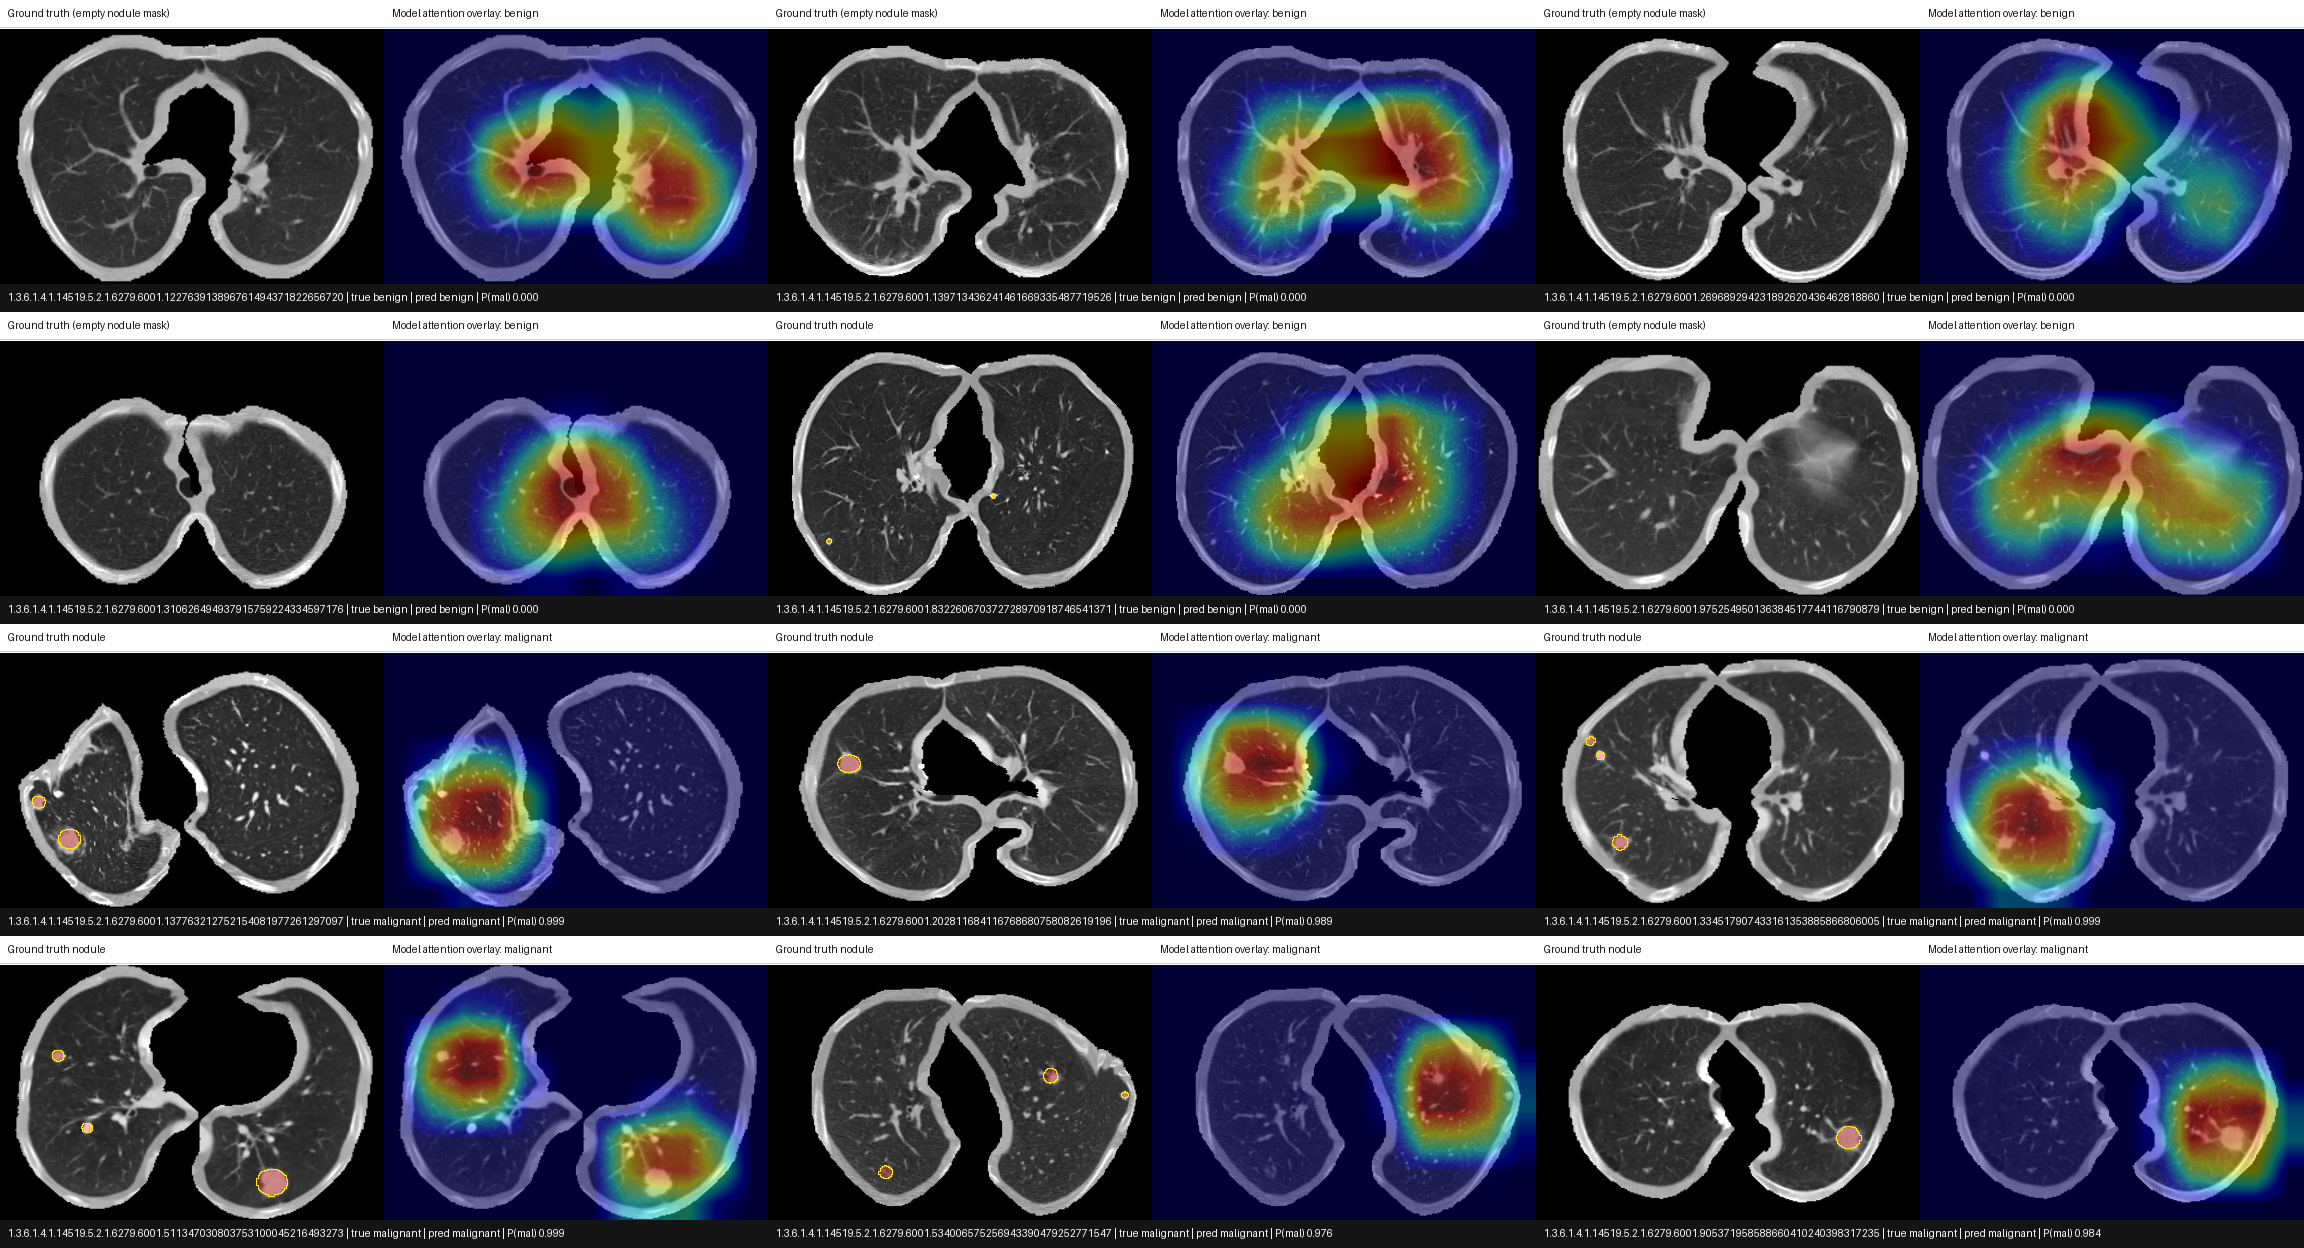
\includegraphics[width=\linewidth]{figures/gradcam_summary.png}
    \caption{
    Grad-CAM interpretability examples for the proposed detector-guided RBF representation.
    The figure shows a class-balanced qualitative subset from the EfficientNetV2-S classifier trained on synthetic 2D images generated with top-$k=4$ detector candidates and a minimum probability threshold of $0.50$.
    For each sample, the left panel shows the ground-truth nodule annotation projected onto the synthetic image, and the right panel shows the Grad-CAM attention overlay for the predicted class.
    Malignant examples are selected among cases where the attention hotspot overlaps the annotated nodule region, illustrating whether the classifier focuses on clinically plausible evidence.
    }
    \label{fig:gradcam_interpretability}
\end{figure}



\subsection{Computational profile}

The proposed representation compresses each preprocessed CT scan into a single $3 \times 256 \times 384$ image. The 3D ResNet18 baseline uses a $1 \times 224 \times 288 \times 288$ volume, corresponding to approximately $63\times$ more scalar input values before accounting for intermediate 3D activations. At the classifier stage, EfficientNetV2-S requires 11.15 GFLOPs for the adaptive 2D image, whereas the 3D ResNet18 forward pass requires 7359.84 GFLOPs. Detector-crop MIL requires up to four 2D encoder passes per patient.

When detector inference is included, the adaptive pipeline is dominated by CPMNetv2 sliding-window inference. CPMNetv2 uses $64 \times 128 \times 128$ crops with stride $48 \times 96 \times 96$, resulting in a mean of 48.40 crops per scan. This corresponds to an average detector-inclusive cost of 33282.75 GFLOPs per scan. This cost should be interpreted as a reusable preprocessing step: the same detections support FROC evaluation, working-point selection, coverage analysis, synthetic generation, and detector-crop baselines.

\section{Discussion}

The results support the central hypothesis that effective 3D-to-2D compression for patient-level malignancy assessment should be lesion-aware. Fixed MIP and central-slice baselines reduce the computational burden, but their sampling geometry is independent of the patient's nodules and therefore dilutes the relevant signal. Fixed-control and random-control RBF ablations further show that the benefit is not explained merely by applying a smooth surface or by using a pretrained 2D backbone. Performance improves only when the surface is guided by detector-derived control points.

The detector-crop MIL baseline addresses an important alternative interpretation: if the detector already localizes nodules, perhaps classifying each candidate independently and aggregating predictions is sufficient. Its lower AUC suggests that the adaptive surface provides useful patient-level context beyond isolated crops. The synthetic image can expose several detected regions and their surrounding anatomy to a single classifier, while still avoiding full-volume inference.

RBF achieved a higher AUC than Shepard interpolation under the selected detector working point. However, the comparison should be interpreted cautiously: the absolute AUC difference was modest and McNemar's test was not significant, indicating that the two interpolation rules produced similar thresholded decision patterns. Thus, Shepard is best viewed as an adaptive interpolation comparator that helps separate the effect of detector-guided sampling from the specific choice of interpolation function, rather than as a clearly inferior alternative.

The computational analysis reveals a nuanced trade-off. If synthetic images and detections are precomputed, the classifier-side cost is comparable to ordinary 2D baselines and far below full-volume 3D classification. If processing begins from raw/preprocessed CT volumes, detector inference dominates the adaptive pipeline. This is not a weakness to hide: the method intentionally uses 3D computation for the task where it is most valuable, localization, and then reuses that intermediate representation for efficient patient-level learning.

\section{Limitations}

This study has several limitations. First, patient-level labels are derived from LIDC-IDRI nodule malignancy ratings rather than from longitudinal clinical outcomes or histopathology, and indeterminate cases were excluded. Second, all experiments were performed on LUNA16/LIDC-derived data; external validation is necessary before clinical claims can be made. Third, the adaptive representation depends on detector quality. Missed nodules or poorly localized candidates can affect the synthesized image. Fourth, although classifier-side inference is efficient, detector-inclusive inference remains computationally expensive because of sliding-window 3D detection. Finally, the current framework synthesizes a single 2D image per scan; future work could study uncertainty-aware multi-surface synthesis or joint optimization of detector and classifier.

\section{Conclusion}

We presented a detection-guided adaptive RBF synthesis framework for patient-level lung malignancy assessment from CT volumes. By converting detector outputs into a smooth patient-specific sampling surface, the method concentrates volumetric nodular evidence into a compact 2D image suitable for efficient classification. On LUNA16, Adaptive RBF with EfficientNetV2-S achieved AUC $0.8149$ and significantly outperformed non-adaptive 2D projections, detector-crop MIL, unguided RBF ablations, Shepard interpolation, and a full-volume 3D ResNet18 baseline. These findings indicate that the key advantage lies not in reducing 3D CT to 2D per se, but in using detector-guided geometry to decide how the reduction is performed.

\section*{Code availability}

The code, experiment scripts, and curated result summaries are available at \url{https://github.com/nico9902/lung_ct_3d2d_synthesis}.

\begin{thebibliography}{99}
\bibitem{carbonneau2018multiple}
M.-A. Carbonneau, V. Cheplygina, E. Granger, and G. Gagnon,
``Multiple instance learning: A survey of problem characteristics and applications,''
\textit{Pattern Recognition}, vol. 77, pp. 329--353, 2018.

\bibitem{nlst2011}
National Lung Screening Trial Research Team,
\newblock Reduced lung-cancer mortality with low-dose computed tomographic screening,
\newblock \emph{New England Journal of Medicine}, 365(5):395--409, 2011.

\bibitem{nelson2020}
H.~J. de Koning et al.,
\newblock Reduced lung-cancer mortality with volume CT screening in a randomized trial,
\newblock \emph{New England Journal of Medicine}, 382(6):503--513, 2020.

\bibitem{armato2011lidc}
S.~G. Armato III et al.,
\newblock The Lung Image Database Consortium (LIDC) and Image Database Resource Initiative (IDRI): A completed reference database of lung nodules on CT scans,
\newblock \emph{Medical Physics}, 38(2):915--931, 2011.

\bibitem{setio2017luna16}
A.~A.~A. Setio et al.,
\newblock Validation, comparison, and combination of algorithms for automatic detection of pulmonary nodules in computed tomography images: The LUNA16 challenge,
\newblock \emph{Medical Image Analysis}, 42:1--13, 2017.

\bibitem{zhu2018deeplung}
W.~Zhu, C.~Liu, W.~Fan, and X.~Xie,
\newblock DeepLung: Deep 3D dual path nets for automated pulmonary nodule detection and classification,
\newblock in \emph{Proc. IEEE Winter Conference on Applications of Computer Vision}, pp.~673--681, 2018.

\bibitem{ardila2019endtoend}
D.~Ardila et al.,
\newblock End-to-end lung cancer screening with three-dimensional deep learning on low-dose chest computed tomography,
\newblock \emph{Nature Medicine}, 25:954--961, 2019.

\bibitem{mikhael2023sybil}
P.~G. Mikhael et al.,
\newblock Sybil: A validated deep learning model to predict future lung cancer risk from a single low-dose chest computed tomography,
\newblock \emph{Journal of Clinical Oncology}, 41(12):2191--2200, 2023.

\bibitem{song2020cpm}
T.~Song et al.,
\newblock CPM-Net: A 3D center-points matching network for pulmonary nodule detection in CT scans,
\newblock in \emph{Medical Image Computing and Computer Assisted Intervention -- MICCAI 2020}, pp.~550--559, 2020.

\bibitem{setio2016multiview}
A.~A.~A. Setio et al.,
\newblock Pulmonary nodule detection in CT images: False positive reduction using multi-view convolutional networks,
\newblock \emph{IEEE Transactions on Medical Imaging}, 35(5):1160--1169, 2016.

\bibitem{zheng2020mip}
S.~Zheng, X.~Cui, M.~Vonder, R.~N.~J. Veldhuis, Z.~Ye, R.~Vliegenthart, M.~Oudkerk, and P.~M.~A. van Ooijen,
\newblock Deep learning-based pulmonary nodule detection: Effect of slab thickness in maximum intensity projections at the nodule candidate detection stage,
\newblock \emph{Computer Methods and Programs in Biomedicine}, 196:105620, 2020.

\bibitem{jang2022m3t}
J.~Jang and D.~Hwang,
\newblock M3T: Three-dimensional medical image classifier using multi-plane and multi-slice transformer,
\newblock in \emph{Proc. IEEE/CVF Conference on Computer Vision and Pattern Recognition}, pp.~20686--20697, 2022.

\bibitem{luo2022scpmnet}
X.~Luo, T.~Song, G.~Wang, J.~Chen, Y.~Chen, K.~Li, D.~N. Metaxas, and S.~Zhang,
\newblock SCPM-Net: An anchor-free 3D lung nodule detection network using sphere representation and center points matching,
\newblock \emph{Medical Image Analysis}, 75:102287, 2022.

\bibitem{powell1987rbf}
M.~J.~D. Powell,
\newblock Radial basis functions for multivariable interpolation: A review,
\newblock in \emph{Algorithms for Approximation}, pp.~143--167, Clarendon Press, 1987.

\bibitem{bookstein1989principal}
F.~L. Bookstein,
\newblock Principal warps: Thin-plate splines and the decomposition of deformations,
\newblock \emph{IEEE Transactions on Pattern Analysis and Machine Intelligence}, 11(6):567--585, 1989.

\bibitem{cantone2025deep}
M. Cantone, C. Russo, F. V. L. Dell'Ascenza, C. Marrocco, and A. Bria,
``Deep learning for DBT classification with saliency-guided 2D synthesis,''
\textit{Pattern Recognition}, p. 112316, 2025.

\bibitem{shepard1968}
D.~Shepard,
\newblock A two-dimensional interpolation function for irregularly-spaced data,
\newblock in \emph{Proceedings of the 1968 23rd ACM National Conference}, pp.~517--524, 1968.

\bibitem{ilse2018attention}
M.~Ilse, J.~M. Tomczak, and M.~Welling,
\newblock Attention-based deep multiple instance learning,
\newblock in \emph{Proceedings of the 35th International Conference on Machine Learning}, PMLR 80:2127--2136, 2018.

\end{thebibliography}

\end{document}
